% This must be in the first 5 lines to tell arXiv to use pdfLaTeX, which is strongly recommended.
\pdfoutput=1
% In particular, the hyperref package requires pdfLaTeX in order to break URLs across lines.

\documentclass[11pt]{article}
\usepackage{enumitem}
% Change "review" to "final" to generate the final (sometimes called camera-ready) version.
% Change to "preprint" to generate a non-anonymous version with page numbers.
\usepackage[review]{acl}
% Standard package includes
\usepackage{times}
\usepackage{latexsym}

% For proper rendering and hyphenation of words containing Latin characters (including in bib files)
\usepackage[T1]{fontenc}
% For Vietnamese characters
% \usepackage[T5]{fontenc}
% See https://www.latex-project.org/help/documentation/encguide.pdf for other character sets

% This assumes your files are encoded as UTF8
\usepackage[utf8]{inputenc}

% This is not strictly necessary, and may be commented out,
% but it will improve the layout of the manuscript,
% and will typically save some space.
\usepackage{microtype}

% This is also not strictly necessary, and may be commented out.
% However, it will improve the aesthetics of text in
% the typewriter font.
\usepackage{inconsolata}

%Including images in your LaTeX document requires adding
%additional package(s)
% \usepackage{graphicx}
\usepackage{graphicx}
\usepackage{xcolor}
\usepackage{tcolorbox}
\usepackage{booktabs}    % 三线表核心宏包
\usepackage{tabularx}    % 自动调整列宽
\usepackage{multirow}    % 多行合并
\usepackage{ragged2e}    % 文本对齐优化
\usepackage{caption}     % 标题格式控制
\captionsetup[table]{skip=5pt, font=small} % 标题样式

% If the title and author information does not fit in the area allocated, uncomment the following
%
%\setlength\titlebox{<dim>}
%
% and set <dim> to something 5cm or larger.

\title{EMO-RL: Emotion-Rule-Based Reinforcement Learning Enhanced Audio-Language Model for Generalized Speech Emotion Recognition}
% EMO-RL: Emotion Rule based Reinforcement Learning for Generalized and Explainable Speech Emotion Recognition


% Author information can be set in various styles:
% For several authors from the same institution:
% \author{Author 1 \and ... \and Author n \\
%         Address line \\ ... \\ Address line}
% if the names do not fit well on one line use
%         Author 1 \\ {\bf Author 2} \\ ... \\ {\bf Author n} \\
% For authors from different institutions:
% \author{Author 1 \\ Address line \\  ... \\ Address line
%         \And  ... \And
%         Author n \\ Address line \\ ... \\ Address line}
% To start a separate ``row'' of authors use \AND, as in
% \author{Author 1 \\ Address line \\  ... \\ Address line
%         \AND
%         Author 2 \\ Address line \\ ... \\ Address line \And
%         Author 3 \\ Address line \\ ... \\ Address line}

\author{First Author \\
  Affiliation / Address line 1 \\
  Affiliation / Address line 2 \\
  Affiliation / Address line 3 \\
  \texttt{email@domain} \\\And
  Second Author \\
  Affiliation / Address line 1 \\
  Affiliation / Address line 2 \\
  Affiliation / Address line 3 \\
  \texttt{email@domain} \\}

%\author{
%  \textbf{First Author\textsuperscript{1}},
%  \textbf{Second Author\textsuperscript{1,2}},
%  \textbf{Third T. Author\textsuperscript{1}},
%  \textbf{Fourth Author\textsuperscript{1}},
%\\
%  \textbf{Fifth Author\textsuperscript{1,2}},
%  \textbf{Sixth Author\textsuperscript{1}},
%  \textbf{Seventh Author\textsuperscript{1}},
%  \textbf{Eighth Author \textsuperscript{1,2,3,4}},
%\\
%  \textbf{Ninth Author\textsuperscript{1}},
%  \textbf{Tenth Author\textsuperscript{1}},
%  \textbf{Eleventh E. Author\textsuperscript{1,2,3,4,5}},
%  \textbf{Twelfth Author\textsuperscript{1}},
%\\
%  \textbf{Thirteenth Author\textsuperscript{3}},
%  \textbf{Fourteenth F. Author\textsuperscript{2,4}},
%  \textbf{Fifteenth Author\textsuperscript{1}},
%  \textbf{Sixteenth Author\textsuperscript{1}},
%\\
%  \textbf{Seventeenth S. Author\textsuperscript{4,5}},
%  \textbf{Eighteenth Author\textsuperscript{3,4}},
%  \textbf{Nineteenth N. Author\textsuperscript{2,5}},
%  \textbf{Twentieth Author\textsuperscript{1}}
%\\
%\\
%  \textsuperscript{1}Affiliation 1,
%  \textsuperscript{2}Affiliation 2,
%  \textsuperscript{3}Affiliation 3,
%  \textsuperscript{4}Affiliation 4,
%  \textsuperscript{5}Affiliation 5
%\\
%  \small{
%    \textbf{Correspondence:} \href{mailto:email@domain}{email@domain}
%  }
%}
\usepackage{amssymb, amsmath, color, framed}
\usepackage{amsmath}
\usepackage{indentfirst} 
\usepackage{multirow}
\begin{document}
\maketitle
\begin{abstract}
	Although Large Audio-Language Models (LALMs) have demonstrated remarkable capabilities in audio perception, their performance in affective computing scenarios, particularly in emotion recognition, reasoning, and subtle sentiment differentiation, remains suboptimal.
	Recent advances in Reinforcement Learning (RL) have shown promise in improving LALMs' reasoning abilities.
	However, two critical challenges hinder the direct application of RL techniques to Speech Emotion Recognition (SER) tasks: (1) convergence instability caused by ambiguous emotional boundaries and (2) limited reasoning ability when using relatively small models (e.g., 7B-parameter architectures).
	To address these challenges, we propose EMO-RL, a novel framework incorporating reinforcement learning with two key innovations: Emotion Similarity-Weighted Reward (ESWR) and Explicit Structured Reasoning (ESR).
	Built upon pretrained LALMs, our method employs group-relative policy optimization with emotion constraints.
	Comprehensive experiments demonstrate that our EMO-RL training strategies can significantly enhance the emotional reasoning capabilities of LALMs, achieving state-of-the-art performance on the MELD and IEMOCAP datasets, and cross-dataset experiments prove the strong superiority of generalization.
\end{abstract}

\section{Introduction}
Speech Emotion Recognition (SER) is a significant research direction in the field of affective computing, aiming to map speech signals to corresponding emotional labels through computational analysis. It plays an important role in various applications, including intelligent customer service~\citep{li2021speech}, mental health assessment~\citep{madanian2022automatic}, and human-computer interaction~\citep{alsabhan2023human}.

\begin{figure}[h]
	\centering
	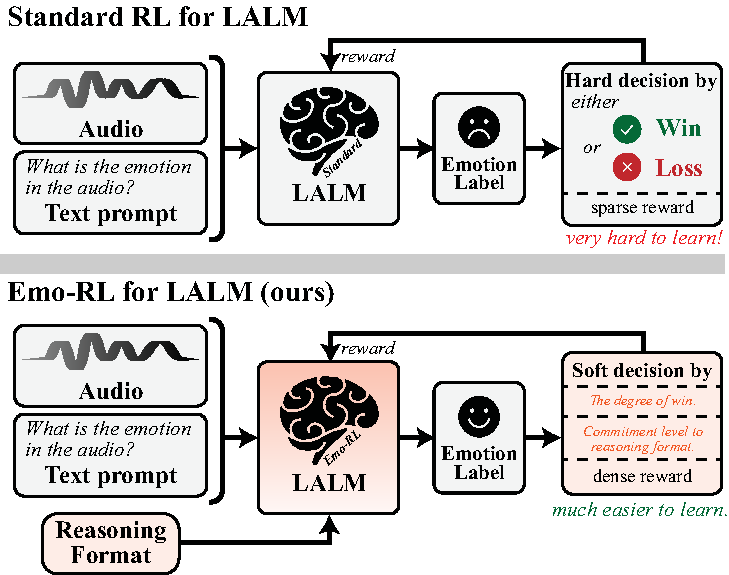
\includegraphics[width=0.49\textwidth]{img/motivation.pdf}
	\caption{The key ideas of our proposed Emo-RL. Compared with the standard RL, Emo-RL exploited emotion similarity-weighted reward and the explicit structured reasoning to improve the emotion recognition performance of LALM.}
	\label{fig:motivation}
\end{figure}

For the SER task, most previous works directly employ speech pre-training models or fine-tune these pre-training models on specific emotional data to extract speech emotional representations, then train a classification head to implement emotion classification~\citep{zou2022speech,chen2023dst,li2024multiscaletemporaltransformerspeech}. However, the emotional representations extracted by these models can only capture the acoustic expressions of emotions, but lack a collaborative analysis of text semantics. These models have very limited generalization capability and lack explainability.

With the development of multi-modal large models, many powerful Large Audio-Language Models (LALMs) have emerged~\citep{kong2024audio,tang2023salmonn}, among which Qwen2-Audio~\citep{chu2024qwen2} is a representative example.
It can follow user instructions to perform many downstream tasks, such as speech recognition, transcription, sound classification, and more. Although Qwen2-Audio demonstrates strong speech understanding capabilities, its performance on SER tasks remains limited.
This limitation stems from its tendency to rely on shallow associations rather than multi-step reasoning that integrates textual semantics and auditory features across modalities, resulting in its limited accuracy and generalization on SER.
Speech emotion recognition inherently constitutes a cognitive reasoning process that necessitates comprehensive analysis from multiple perspectives through step-by-step reasoning.
When humans recognize emotions in speech, they often understand the specific content and keywords of speech and integrate this understanding based on acoustic features (such as pitch level, speech rate, energy intensity, voice quality).
For example, when someone says "fed up" with rapid speech, high volume, and sharp intonation, anger can be inferred.

These reasoning steps are beyond the capability of traditional audio feature extraction and classification head frameworks.
Extensive research has shown that reinforcement learning can enhance the reasoning capabilities of LLM~\citep{guo2025deepseek,team2025kimi}.
% However, currently, there is no reinforcement learning framework specifically designed for LALM for speech emotion tasks. 
The effective deployment of reinforcement learning (RL) in SER encounters two fundamental limitations: convergence reliability issues primarily arising from ill-defined inter-class affective boundaries that induce gradient conflict during policy updates, compounded by insufficient affective reasoning capacity in under-parameterized architectures (e.g., 7B-parameter configurations).

To address these challenges, we adopt a psychological perspective by transforming the original right/wrong classification problem into a regression problem that accommodates varying degrees of correctness and error, through the introduction of an emotion-state-transition matrix (As illustrated in Figure~\ref{fig:motivation}).
We implement an Emotion Similarity-Weighted Reward (ESWR) mechanism that progressively guides the policy model from simpler to more complex tasks. This approach initially teaches the model to distinguish between basic positive and negative emotions before advancing to finer-grained emotional distinctions.
To further enhance the model's emotional reasoning capabilities, we incorporate Explicit Structured Reasoning (ESR) strategies  during RL training. These strategies provide the model with guiding clues to help it more effectively differentiate between emotions, thereby improving its overall reasoning performance in speech emotion recognition tasks.

Based on the ESWR and ESR, we exploited our emotion-rule-based RL method to fine-tune the LALM, and achieved better emotion recognition performance compared with current state-of-the-art methods.
The contributions of this paper are as follows:
\begin{itemize} [leftmargin=10pt]
	\item We propose a speech emotion recognition pipeline via RL fine-tuning of a large audio and language model.
	\item We introduce Emotion-rule based RL to improve the emotion recognition ability of LALM, leveraging emotion similarity-weighted rewards and explicit structured reasoning strategies.
	\item Extensive experiments show that our method achieves state-of-the-art performance and exhibits strong generalizability.
\end{itemize}
\section{Related Works}
\subsection{Generalized Speech Emotion Recognition}

For speech emotion recognition, traditional approaches have focused on designing novel network architectures~\citep{zou2022speech, chen2023dst, li2024multiscaletemporaltransformerspeech} based on classical neural networks such as CNN, LSTM, and Transformer.
With the advancement of self-supervised learning, researchers have increasingly utilized pre-trained audio models like HuBERT~\citep{hsu2021hubert}, WavLM~\citep{chen2022wavlm}, Emotion2vec~\citep{ma2023emotion2vec}, and Whisper~\citep{radford2023robust} to extract speech features or fine-tune these models on speech emotion datasets to obtain emotion-specific features~\citep{morais2022speech, chen2023exploring}.
Subsequently, a linear classification head is trained to perform emotion classification.
These models, pre-trained on large-scale and diverse speech corpora, have significantly enhanced speech emotion perception capabilities~\citep{li2023exploration}.
For instance, the Vesper model~\citep{chen2024vesper}, obtained by distilling the WavLM-large model with emotion data, has achieved promising results in speech emotion recognition tasks.
% Emotion2vec~\citep{ma2023emotion2vec} presents the first universal speech emotion representation model, pre-trained on open-source unlabeled emotion data through self-supervised online distillation, combining utterance-level loss and frame-level loss during pre-training. 
However, the generalization capabilities of these models remain limited, and they lack collaborative analysis of text semantics and explainability.
% Currently, there is no research using LALM and reinforcement learning methods specifically for the SER task.

\subsection{Large Audio-Language Models}
Recent advances in multi-modal large language models have led to the emergence of numerous LALMs, such as Qwen2-Audio~\citep{chu2024qwen2}, Audio Flamingo~\citep{kong2024audio}, and SALMONN~\citep{tang2023salmonn}, which have demonstrated strong audio understanding capabilities, with Qwen2-Audio even outperforming previous systems on nearly all audio-centric benchmarks.
These models typically comprise three main components: an Audio Encoder, a Large Language Model, and a modality connector that bridges them.
% LALMs are typically trained using a multi-stage training framework of pre-training and supervised fine-tuning. 
% They can directly process cross-modal inputs of audio (speech, environmental sounds, music, etc.) and text prompts, as well as generate textual outputs. 
% They can follow user instructions to perform many downstream tasks, such as speech recognition, transcription, sound classification, and more.
These models are capable of directly processing cross-modal inputs, including audio (such as speech, environmental sounds, and music) and text prompts, and can generate the corresponding textual output. They are able to follow user instructions to perform a variety of downstream tasks, such as speech recognition, transcription, and sound classification~\citep{wang2025enabling, waheed2024speech}.
% Unlike simple descriptive tasks like Automatic speech recognition (ASR) or automated audio captioning (AAC), one of the unique and most promising capabilities of LALMs is the Audio Question Answering (AQA) task. 
% AQA is a more advanced and challenging multi-modal task that involves understanding and reasoning based on audio content to generate accurate answers. 
% It integrates auditory and language modalities, requiring complex logical reasoning abilities from the model. 
% However, these models are primarily trained for perception and straightforward QA tasks. They do not incorporate explicit multi-step reasoning or chain-of-thought during training. Consequently, The capabilities of LALM like Qwen2-Audio can be further stimulated in complex audio reasoning tasks such as SER. It is critical to enhance the reasoning ability of LALM.
However, current LALM training mainly focuses on perception and basic QA tasks, lacking explicit multi-step reasoning. Thus, the potential of LALMs like Qwen2-Audio in complex audio reasoning tasks such as SER remains untapped. Enhancing their reasoning abilities in these advanced tasks is crucial.

\subsection{Reinforcement Learning and Reasoning}
Reinforcement learning (RL) is pivotal for enhancing the reasoning capabilities of LLMs and MLLMs.
RL from human feedback (RLHF) aligns LLMs using proximal policy optimization (PPO)~\citep{schulman2017proximal} and a learned reward model.
DPO~\citep{rafailov2023direct} learns directly from preferences without reward models, while RFT~\citep{yuan2023scaling} enhances reasoning via filtered self-generated traces.
GRPO~\citep{shao2024deepseekmath} improves upon PPO by removing the critic and using group-averaged baselines for advantage estimation, boosting LLM reasoning with lower complexity.
Hybrid GRPO~\citep{sane2025hybrid} combines GRPO’s sampling with a learned value function, enhancing stability and sample efficiency.

Recent studies indicate that COT and RL can enhance the reasoning performance of LALM. Audio-CoT~\citep{ma2025audio} first applied CoT to LALMs but had limited improvement due to no parameter updates.
Audio-Reasoner~\citep{xie2025audio} introduced a large synthetic dataset (CoTA) with over a million QA pairs and step-by-step reasoning annotations, which significantly improved long-context reasoning performance.
Xiaomi used the GRPO algorithm to fine-tune the Qwen2-Audio-7B model on audio QA tasks~\citep{li2025reinforcement}, enhancing reasoning accuracy.
% The RL-based approach effectively improved reasoning accuracy, suggesting that reward-driven optimization can extract more signal from limited training examples. 
SARI~\citep{wen2025sari} further integrates structured reasoning with curriculum-guided reinforcement learning, achieving state-of-the-art performance on the MMAU and MMSU benchmarks.
The RL-based approach effectively improved reasoning accuracy, suggesting that reward-driven optimization can extract more signal from limited training examples. However, these RL-based methods are too generalized for direct application to speech emotion tasks. Thus, we need to explore SER tasks using emotion-rule-based reinforcement learning.

\section{Methodology}
\begin{figure*}[h]
	\centering
	% \includegraphics[width=1\textwidth]{latex/img/framework.pdf}
	\includegraphics[width=0.99\linewidth]{./img/framework.pdf}
	\caption{The overview of the Emo-RL for LALM to improve the generalized speech emotion recognition. Building on GRPO, we enhance emotion recognition via two improvements. First, we create an emotion-state-transition matrix from Plutchik's wheel of emotions~\cite{plutchik1982psychoevolutionary}, allowing the policy model to receive rewards for predicting similar emotions. Second, we introduce explicit structured reasoning to directly input human emotion recognition priors into the model.}
	\label{fig:main_figure}
	\vspace{-0.5cm}
\end{figure*}

\subsection{Problem Definition}
We use emotional audio question answering in Qwen2-Audio-7B-Instruct to implement SER.
SER process through LALMs constitutes a parametric mapping process where: given a speech signal $x$ and structured textual query $Q$ containing multiple-choice options, their temporal-contextual concatenation forms the input prompt $p=[x;Q]$. The LALM, $\pi_{\boldsymbol{\theta}}$, then generates emotion prediction $\hat{y}$ through cross-modal understanding, formally expressed as:
% Specifically, SER by LALM can be formally defined as follows: given a speech input $S$ and a customized template textual multiple-choice question $Q$, which construct the prompt, the LALM, $f_{\theta}$, could generate the emotion label $Y$, denoted as the equation~\ref{forward}.
\begin{equation}
	\pi_{\boldsymbol{\theta}}(x; Q)\to a \to \hat{y},
	\label{forward}
\end{equation}
where $S$ is a speech audio with a sampling rate of 16kHz, $Q$ is the textual question prompt, and $a$ is the generated response of LALM, including thinking and reasoning contents and the final selected answer, and $\hat{y}$ denotes the predicted emotion label.

This study aim to address two core challenges in SER through LALMs: (1) Enhancing the predictive accuracy of $f_\theta$ via reinforcement learning using the training dataset $\mathcal{D}=\{(x_{i}, y_{i})\}^{N}_{i}$, where the N means the sample number. (2) Discovering optimal prompt formulations $Q$ to improve the inference performance. Considering the parameter space of is infinite, we defined three experimentally validated designs as the Q space, $\mathbf{Q}$, including implicit reasoning $Q_{\mathrm{IR}}$, explicit unstructured reasoning $Q_{\mathrm{EUR}}$, explicit structured reasoning $Q_{\mathrm{ESR}}$. Therefore, the target of this study could be defined as:
\begin{equation}
	\theta, Q = \arg \max_{\theta, Q \in \mathbf{Q}} (\mathcal{R}(\pi_{\boldsymbol{\theta}}(X;Q), Y)),
	\label{object}
\end{equation}
where the $R$ denotes the reward function.
% Its task is to identify the correct answer option $A$ from N candidate options in tag <Choices> by analyzing and reasoning through the information in the speech input. This process can be represented as a mapping:

% where $S$ is a speech audio with a sampling rate of 16kHZ, $Q$ is the textual question prompt, and $A$ is the derived answer, including thinking and reasoning contents and the final selected answer. Through this mapping, LALM integrates speech audio and textual prompts to achieve effective emotional reasoning.

In detail, we explore three reasoning strategies in
EMO-RL training to evaluate the impact of reasoning patterns. We detail three patterns below:
\begin{itemize}[leftmargin=10pt]
	\item Implicit Reasoning, $Q_{\mathrm{IR}}$: As a baseline, we fine-tune the model only to output the final answer, without requiring the model to explicitly output its reasoning process.
	\item Explicit Unstructured Reasoning, $Q_{\mathrm{EUR}}$: To model more free-form, naturalistic reasoning, we prompt the model without imposing any predefined structure or sectioning. Although unstructured, the model is required to produce a coherent explanation that ends with a definitive answer.
	\item Explicit Structured Reasoning, $Q_{\mathrm{ESR}}$: We attempt the model to output a clear and structured chain-of-thought. The model is prompted to produce the two-section reasoning format, including speech content (text transcription, keywords) and acoustic features (pitch level, speech rate, energy intensity, voice quality). Combining the above two aspects of information, the model outputs the final answer.
\end{itemize}

\subsection{Emotion-rule based RL framework}
We built our Emo-RL based on the GRPO framework for its efficiency and scalability. Unlike proximal policy optimization, which requires a computationally expensive value network, GRPO calculates relative advantages by comparing rewards within a group of sampled actions, reducing computational overhead and simplifying optimization. This makes GRPO particularly suitable for speech reasoning tasks. Similar to GRPO, the Emo-RL also has three main steps, sampling action groups, reward evaluation, and updating policy network with relative advantage and KL divergence (As shown in Figure~\ref{fig:main_figure}).

\textbf{Sampling Action Groups} For each input state $s=(x,Q)$ , where $x$ is the speech encoding of the input audio and $Q$ the textual encoding of the question, GRPO samples a group of actions (the generated response of LALM), $\{a_{1},a_{2},\ldots,a_{G}\}$, from the current policy $\pi_{\boldsymbol{\theta}}$. The sampling process is:
\begin{equation}
	a_{i}\sim\pi_{\theta}(a\mid x,Q),\quad{\mathrm{for}}\quad i=1,2,\ldots,G.
\end{equation}
This strategy ensures diverse responses, promoting exploration and preventing premature convergence.

\textbf{Reward Evaluation}. In our reinforcement learning framework, each sampled action $a_{i}$ is assigned a reward $\mathcal{R}(a_{i})$ based on verifiable criteria, resulting in a reward set $\{r_{1},r_{2},\dots,r_{G}\}$. For emotional speech reasoning tasks, the reward function $\mathcal{R}(a_{i})$ combines two components: the Explicit Structured Reasoning Reward (ESR) $\mathcal{R}_{\mathrm{ESR}}(a_{i})$ and Emotion Similarity-Weighted Reward (ESWR), $\mathcal{R}_{\mathrm{ESWR}}(a_{i})$. The ESR ensures that the responses adhere to a structured format, thereby guiding the reasoning strategy of the policy network, $\pi_{\theta}$. The ESWR evaluates the correctness of the action $a_{i}$, providing feedback to $\pi_{\theta}$ on the extent to which the answer aligns with the correct response. The overall reward function is formally defined as:
\begin{equation}
	\mathcal{R}(a_{i})=\mathcal{R}_{\mathrm{ESWR}}(a_{i})+\mathcal{R}_{\mathrm{ESR}}(a_{i}).
\end{equation}

\textbf{Updating Policy Network with Relative Advantage and KL divergence}. The $\pi_{\theta}$ is optimized by the Relative Advantage of rewards and KL divergence between $\pi_{\theta}$ and reference model $\pi_{\mathrm{ref}}$. Firstly, policy Rewards are normalized within the sampled group to compute relative advantages $\{A_{1},A_{2},\dotsc,A_{G}\}$, defined as:
\begin{equation}
	A_{i}={\frac{r_{i}-\operatorname*{mean}\{r_{1},r_{2},\ldots,r_{G}\}}{\operatorname{std}\{r_{1},r_{2},\ldots,r_{G}\}}}.
\end{equation}
Based on these advantages, the policy is updated to reinforce actions with positive advantages and reduce the probability of less effective ones. To ensure stable RL learning, $\pi_{\theta}$ updates are further constrained by minimizing the KL divergence between the updated and reference models.
% The we have objective function as below:
% \begin{equation}
% \begin{align}
% \tiny
% J(\theta) = \mathbb{E}_{q, \{a_i\}_{i=1}^{G}} \\
% \left[ \sum_{t=1}^T \min\left( \frac{\pi_\theta(a_{i,t}|o_{i,t}, q)}{\pi_{\mathrm{old}}(a_{i,t}|o_{i,t}, q)} \cdot r(a_i), \mathrm{clip}\left( \frac{\pi_\theta(a_{i,t}|o_{i,t}, q)}{\pi_{\mathrm{old}}(a_{i,t}|o_{i,t}, q)}, 1-\epsilon, 1+\epsilon \right) \cdot r(a_i) \right) \right] 
% - \beta D_{\mathrm{KL}}[\pi_\theta \| \pi_{\mathrm{old}}]
% \end{align}
% \end{equation}


\subsection{Rewards Mechanism Design}
% There are two reward functions in EMO-RL, accuracy reward and format reward. Responses are evaluated by a rule-based reward function in terms of their format and correctness.
The EMO-RL framework implements dual reward mechanisms synergistically combining structural compliance enforcement and affective alignment optimization.
Specifically, domain-specific response schemata are enforced through regular-expression pattern matching that validates three distinct reasoning pattern compliance rates ($Q_{\text{IR}}, Q_{\text{EUR}}, Q_{\text{ESR}}$), systematically enhancing explainability via cognitive transparency in decision pathways.
Complementarily, the emotion similarity-weighted reward employs an emotion-state-transition matrix constructed through Plutchik's wheel of emotions~\cite{plutchik1982psychoevolutionary}, generating dense reward signals that precisely guide policy gradients through convex optimization landscapes.
% For format rewards, we have designed three corresponding format reward functions targeting our three reasoning prompts, ensuring that the model strictly adheres to structured response formats. This significantly improves explainability and consistency. For accuracy rewards, we propose an emotion similarity-weighted reward function that utilizes more fine-grained and dense reward signals, which are more aligned with psychological principles while making gradient update directions more precise, thereby accelerating convergence.
\subsubsection{Explicit Structured Reasoning Reward}
This component ensures structured and explainable responses by requiring the model to follow predefined templates: reasoning between \texttt{<think>} and \texttt{</think>} tags, and providing the final answer between \texttt{<answer>} and \texttt{</answer>} tags. Strict format adherence earns a reward score of 1, while deviation results in a reward score of 0. A binary reward is assigned based on a regular-expression (regex) pattern matching.
\begin{equation}
	\mathcal{R}_{\mathrm{ESR}}=\begin{cases}1,&\text{if the format matches $Q_{\text{ESR}}$}   \\ 0, &\mathrm{otherwise.}\end{cases}
\end{equation}
\subsubsection{Emotion Similarity-Weighted Reward}
The conventional approach uses binary classification rewards, assigning a score of 1 for completely correct answers and 0 otherwise. However, this has limitations when applied to emotions, as it ignores the relationships between different emotion types. Emotions are inherently continuous and complex. Drawing from psychological emotion dimension theories~\cite{plutchik1982psychoevolutionary} and other psychological knowledge, we comprehensively consider emotion valence (the positive or negative of emotions) and arousal (the intensity or activation level of emotions). We have meticulously designed an emotion-state-transition matrix $S \in \mathbb{R}^{C \times C}$ ($C$ denote emotion categories) as:
% how to construct the matrix
% \begin{equation}
% % \small
%     S_{i,j} =
% \begin{cases}
% 0.5, \quad \text{if $y_{i}$ or $y_{j}= $`neutral'}, \\
% \frac{1}{2}(\cos(\mathrm{Plutchik}(y_{i}, y_{j})+1), \mathrm{otherwise.}
% \end{cases}
% \end{equation}

\begin{equation}
	\begin{footnotesize}
		S_{i,j}=\left\{ \begin{matrix}
			\frac{1}{2},                                                                       & \text{if $y_i$ or $y_i$=`$\mathrm{neutral}$'} \\
			\frac{1}{2}\left( \cos \left( \text{Pl}\left( y_i,y_j \right) \right) +1 \right) , & \mathrm{otherwise}                            \\
		\end{matrix} \right.
	\end{footnotesize}
\end{equation}


Here, the $y_{i}$ and $y_{j}$ denotes two emotion types, and $\mathrm{Pl}(\cdot, \cdot)$ means the angles from each other on the Plutchik's wheel of emotions.
Based on the $S$, we have the Emotion Similarity-Weighted Reward function, formulated as:
% $$\mathcal{R}_{\mathrm{acc}} =
% \begin{cases}
% 1 & \mathrm{Full match} \\
% \alpha \cdot S(y_{\mathrm{pred}}, y_{\mathrm{true}}) & \mathrm{Partial match} \\
% -\beta & \mathrm{Contradictory emotions}
% \end{cases}$$
\begin{equation}
	\mathcal{R}_{\mathrm{ESWR}} =
	\begin{cases}
		1                          & S(\hat{y}, y) = 1     \\
		\alpha \cdot S(\hat{y}, y) & S(\hat{y}, y)>\gamma  \\
		0                          & S(\hat{y}, y)<=\gamma
	\end{cases}
\end{equation}
where $\alpha$ is the partial matching coefficient, dynamically adjusting from 1 to 0 during training, and $\gamma$ is the threshold of the contradictory emotion, which was set as 0.7 in this paper.

% \begin{tcolorbox}[myframe]
% \noindent
% \color{black} % 文本颜色为白色
% \textbf{Prompts for EMO-RL}

% \begin{description}
% \item[Implicit Reasoning:] 
% What is the emotion of the speaker in the audio? Please choose the answer from the following options: |<Choices>|. Output the final answer in <|FunctionCallBegin|> </RichMediaReference>.

% \item[Explicit Structured Reasoning:] 
% What is the emotion of the speaker in the audio? Output the thinking process in <RichMediaReference> </RichMediaReference>. Please choose from the following options: |<Choices>| and output final answer in <RichMediaReference> </RichMediaReference>.  

% \item[Explicit Unstructured Reasoning:] 
% What is the emotion of the speaker in the audio? First analyze the speaker's speech content in <think1> </think1>, then analyze the speaker's acoustic features in <think2> </think2>. After that, choose from the following options: |<Choices>| and output final answer in <RichMediaReference> </RichMediaReference>. 
% \end{description}
% \end{tcolorbox}

\section{Experiment}
\subsection{Experimental Setup}
\subsubsection{Dataset}
We evaluate model capabilities and generalization in speech emotion recognition (SER) using four datasets:
\begin{itemize}[leftmargin=10pt]
	\item
	      \textbf{MELD}~\citep{poria2018meld}: Contains 13,708 utterances from \emph{Friends}, classified into seven emotions. It tests model performance in noisy, complex environments.
	\item
	      \textbf{IEMOCAP}~\citep{busso2008iemocap} is the most widely used dataset for SER tasks. To maintain consistency and comparability with previous methods and benchmark~\citep{ye2023temporal,ma2024emobox}, we focus on 5,531 utterances from four emotions: Angry, Neutral, Happy, and Sad.
	\item
	      \textbf{RAVDESS}~\citep{livingstone2018ryerson} is an emotional database containing 4,800 samples, including audio-video data of speech and songs for emotion recognition research. It encompasses 8 emotions: Neutral, Calm, Happy, Sad, Angry, Fearful, Surprised, and Disgusted.
	\item
	      \textbf{SAVEE}~\citep{jackson2014surrey}: Contains 480 samples with natural and exaggerated expressions of seven emotions, including Anger, Disgust, Fear, Happy, Sad, Surprise, and Neutral.

\end{itemize}

% IEMOCAP~\citep{busso2008iemocap} is the most widely used dataset for SER tasks. To maintain consistency and comparability with previous methods and benchmark~\citep{ye2023temporal,ma2024emobox}, we focus on 5,531 utterances from four emotions: Angry, Neutral, Happy, and Sad.
% RAVDESS~\citep{livingstone2018ryerson} is an emotional database containing 4,800 samples, including audio-video data of speech and songs for emotion recognition research. It encompasses 8 emotions: Neutral, Calm, Happy, Sad, Angry, Fearful, Surprised, and Disgusted.
% SAVEE~\citep{jackson2014surrey} is an emotion dataset that contains 480 samples, featuring natural and exaggerated expressions of various emotions. It includes 7 emotions: 

\subsubsection{Implementation Details}
We use Qwen2-Audio-7B-instruct as the foundational backbone model for our experiments.
The RL models are trained using eight NVIDIA RTX 4090 GPUs, with each device running a batch size of 1 and Gradient Accumulation Steps set to 2.
The model is trained for 300 steps with a learning rate of $1 \times 10^{-6}$ and a temperature of 1.0.
Each reinforcement learning optimization step generates 6 responses per sample.
The SFT models use the AdamW optimizer with a learning rate of $1 \times 10^{-5}$ and are trained for a total of 5 epochs.
The optimal iteration results are selected for final analysis.

\subsubsection{Baselines and Metrics}
We compare our method with state-of-the-art (SOTA) approaches, categorized into three types: \textbf{W/o-LALM}, \textbf{LALM}, and \textbf{LALM-FT}.
W/o-LALM and LALM-FT refer to models post-trained on the MELD training set, while LALM involves zero-shot inference using prompt strategies without task-specific fine-tuning.
\begin{itemize}[leftmargin=10pt]
	\item \textbf{W/o-LALM}: We selected four advanced self-supervised pre-trained audio models: HuBERT large~\cite{hsu2021hubert}, WavLM large~\cite{chen2022wavlm}, data2vec 2.0 large~\cite{baevski2023efficient}, Whisper large v3~\cite{radford2023robust} and Emotion2vec~\cite{ma2023emotion2vec}. Features from the last Transformer layer of these frozen pre-trained models were extracted to train the downstream linear layers with a hidden dimension of 256.
	\item \textbf{LALM}: We directly use Qwen2-Audio~\cite{chu2024qwen2} for SER tasks without additional training or fine-tuning, employing two prompt patterns: direct inference and chain-of-thought inference.
	\item \textbf{LALM-FT}: We further trained Qwen2-Audio. To evaluate different training methods, we compare models trained with supervised fine-tuning (SFT), GRPO~\cite{shao2024deepseekmath}, and EMO-RL. Additionally, we assess the impact of different reasoning strategies in EMO-RL: implicit reasoning, unstructured explicit reasoning, and structured explicit reasoning.
\end{itemize}
In our evaluation, we utilize three key metrics: Weighted Accuracy (WA), Unweighted Accuracy (UA), and Macro F1 Score (F1), to assess the performance of the speech emotion recognition task. WA reflects the overall accuracy of the model across all emotion classes.
UA measures the average accuracy by considering each emotion class equally, regardless of its frequency in the dataset.
The F1, which combines precision and recall, provides a robust evaluation of model performance, particularly in scenarios where there is an imbalance in the distribution of emotion classes.

\begin{table*}[ht]
	\caption{The comparison of the main performance metrics for various methods on the MELD and IEMOCAP datasets. Results for W/o-LALM methods are cited from the Emobox benchmark~\cite{ma2024emobox} and~\cite{ma2023emotion2vec}.
		The \textbf{bold} font indicates the best results among all models.
		The baseline here denotes the GRPO+IR, and the SOTA means the best results among W/o-LALM methods.}
	\label{tab:performance}
	\centering
	\small
	\setlength{\tabcolsep}{2.4pt}

	\begin{tabularx}{\textwidth}{>{\raggedright\arraybackslash}p{1.55cm} llccccccc} % 分为两组3列
		\toprule
		\multirow{2}{*}{\textbf{Model Type}} & \multirow{2}{*}{\textbf{Model}}                   & \multirow{2}{*}{\textbf{Method}} & \multicolumn{3}{c}{\textbf{MELD}} & \multicolumn{3}{c}{\textbf{IEMOCAP}}                                                                                                                                             \\
		\cmidrule(r){4-6} \cmidrule(l){7-9} % 分割线
		                                     &                                                   &                                  & \textbf{UA($\%$)}                 & \textbf{WA($\%$)}                    & \textbf{F1($\%$)}                & \textbf{UA($\%$)}                & \textbf{WA($\%$)}                & \textbf{F1($\%$)}                \\
		\midrule
		\multirow{4}{*}{\mathrm{W/o-LALM} }
		                                     & HuBERT large~\citep{hsu2021hubert}                & Classification Head              & 24.13                             & 46.37                                & 24.99                            & 67.42                            & 66.69                            & 67.24                            \\
		                                     & WavLM large~\citep{chen2022wavlm}                 & Classification Head              & 28.18                             & 49.31                                & 29.11                            & 69.47                            & 69.07                            & 69.29                            \\
		                                     & data2vec 2.0 large~\citep{baevski2023efficient}   & Classification Head              & 26.33                             & 47.72                                & 27.35                            & 57.30                            & 56.23                            & 56.70                            \\
		                                     & Whisper large V3~\citep{radford2023robust}        & Classification Head              & 31.54                             & 51.89                                & 32.95                            & 73.54                            & 72.86                            & 73.11                            \\
		                                     & Emotion2vec+ large~\citep{ma2023emotion2vec}      & Classification Head              & 28.03                             & 51.88                                & /                                & 70.70                            & 67.30                            & /                                \\
		\midrule
		\multirow{2}{*}{LALM}
		                                     & \multirow{2}{*}{Qwen2-Audio~\cite{chu2024qwen2}}  & Direct Inference                 & 18.96                             & 39.83                                & 19.84                            & 53.76                            & 51.52                            & 47.68                            \\
		                                     &                                                   & CoT Inference                    & 26.89                             & 50.57                                & 28.05                            & 64.33                            & 60.37                            & 61.61                            \\
		\midrule

		\multirow{5}{*}{LALM-FT}
		                                     & \multirow{5}{*}{Qwen2-Audio~\cite{chu2024qwen2}}
		                                     & SFT + IR                                          & 33.26                            & 57.39                             & 35.77                                & 85.70                            & 83.87                            & 84.53                                                               \\
		                                     &                                                   & GRPO + IR                        & 31.60                             & 55.41                                & 33.22                            & 81.74                            & 80.00                            & 80.71                            \\
		                                     &                                                   & + ESWR + IR                      & 36.23                             & 63.85                                & 38.57                            & 84.12                            & 83.90                            & 83.11                            \\
		                                     &                                                   & + ESWR + EUR                     & 37.81                             & 66.17                                & 39.19                            & 85.97                            & 84.85                            & 85.50                            \\
		                                     &                                                   & + ESWR + ESR                     & \textbf{39.46}                    & \textbf{69.56}                       & \textbf{41.87}                   & \textbf{87.42}                   & \textbf{87.28}                   & \textbf{87.40}                   \\
		\midrule
		\multirow{2}{2}{/}                   & \multirow{2}{*}{Comparason}
		                                     & Ours VS SOTA                                      & \textcolor{teal}{$\uparrow$25.1} & \textcolor{teal}{$\uparrow$34.0}  & \textcolor{teal}{$\uparrow$27.1}     & \textcolor{teal}{$\uparrow$18.9} & \textcolor{teal}{$\uparrow$19.8} & \textcolor{teal}{$\uparrow$19.6}                                    \\
		                                     &                                                   & Ours VS Baseline                 & \textcolor{teal}{$\uparrow$24.9}  & \textcolor{teal}{$\uparrow$25.5}     & \textcolor{teal}{$\uparrow$26.0} & \textcolor{teal}{$\uparrow$6.95} & \textcolor{teal}{$\uparrow$10.9} & \textcolor{teal}{$\uparrow$10.8} \\

		\bottomrule
	\end{tabularx}
\end{table*}

\subsection{Main Performance}
As shown in Table~\ref{tab:performance}, the results demonstrate the effectiveness of COT in LALM, our proposed ESWR, and ESR.
\textbf{Effectiveness of COT in LALM}: Using CoT prompts significantly enhances the zero-shot SER performance of LALMs. In fact, CoT enables Qwen2-Audio to approach the performance of the best W/o-LALM pre-trained audio models without any task-specific post-training.
\textbf{Effectiveness of ESWR}: When training and testing on the same dataset, the direct use of GRPO achieves similar accuracy to SFT. This may be due to the MELD dataset containing considerable noise, resulting in the model's lower ability to recognize correct emotions. This leads to GRPO's binary rewards being too sparse, with 60\% of accuracy rewards being 0, making it difficult for the model's update policy to stabilize. However, ESWR provides more dense and psychologically grounded reward signals, improving the model's emotional reasoning capability by consistently guiding it toward the correct emotional direction.

\textbf{The effectiveness of ESR training strategies}. Besides the ESWR method, compared to models trained with IR, models trained with EUR and ESR can both enhance emotional reasoning capabilities, improving accuracy on the MELD and IEMOCAP test sets. Moreover, models with structured thinking capabilities achieve higher accuracy than those with unstructured thinking capabilities, indicating that structured reasoning helps models avoid errors.
Through the above experiments, we have demonstrated that using the EMO-RL algorithm can significantly enhance the emotional reasoning capabilities of LALMs, achieving state-of-the-art performance in speech emotion recognition tasks. Additionally, we found that our method yields greater improvements on datasets with more complex emotion labels, for example, the improvement of MELD, compared to IEMOCAP.

\begin{table}[t]
	\caption{Weighted Accuracy (WA, \%) across RAVDESS, SAVEE, and IEMOCAP Datasets. The model was trained on the MELD training dataset. The baseline here denotes the SFT+IR.}
	\label{tab:multi-dataset}
	\centering
	\small
	\setlength{\tabcolsep}{4.2pt}
	\begin{tabularx}{0.49\textwidth}{llccc}
		\toprule
		\textbf{Model}     & \textbf{RAVDESS}                  & \textbf{SAVEE}                    & \textbf{IEMOCAP}                 \\
		\midrule
		\multicolumn{5}{l}{\textit{W/o-LALM Baselines}}                                                                               \\
		% \midrule
		HuBERT large       & 25.02                             & 31.54                             & 44.60                            \\
		WavLM large        & 33.90                             & 34.10                             & 48.59                            \\
		data2vec 2.0 large & 34.21                             & 37.79                             & 47.43                            \\
		Whisper large v3   & 40.68                             & 42.18                             & 46.14                            \\
		\midrule

		\multicolumn{5}{l}{\textit{LALM-FT (Qwen2-Audio~\cite{chu2024qwen2})}}                                                        \\
		% \multirow{5}{*}{}
		% \midrule
		SFT+ IR            & 59.83                             & 71.52                             & 82.74                            \\
		GRPO + IR          & 62.07                             & 72.38                             & 82.66                            \\
		+ ESWR + IR        & 66.21                             & 74.69                             & 83.05                            \\
		+ ESWR + EUR       & 70.43                             & 78.57                             & 86.11                            \\
		+ ESWR + ESR       & \textbf{73.99}                    & \textbf{80.83}                    & \textbf{87.86}                   \\
		\midrule
		Ours VS Baseline   & \textcolor{teal}{$\uparrow$23.67} & \textcolor{teal}{$\uparrow$13.02} & \textcolor{teal}{$\uparrow$6.19} \\
		\bottomrule
		\vspace{-0.5cm}
	\end{tabularx}
\end{table}

\subsection{Generalizability}
In practical scenarios, a model's ability to generalize emotion recognition to unseen individuals and unknown recording conditions is of paramount importance.
To evaluate this capability, cross-dataset zero-shot testing offers an effective means of assessing a model's generalization in emotion recognition.
We meticulously selected three diverse datasets: IEMOCAP, RAVDESS, and SAVEE.
These datasets encompass a variety of sources, accents, and recording environments, enabling a comprehensive evaluation of the model's generalization and robustness across real-world scenarios.

As shown in Table~\ref{tab:multi-dataset}, the results of cross-datasets evaluation demonstrate that \textbf{(1)} Reinforcement learning methods, including GRPO and ESWR, demonstrate superior generalization capabilities compared to SFT methods. Notably, ESWR exhibits better generalization than GRPO. Additionally,
\textbf{(2)} Explicit Reasoning strategies show enhanced generalization over Implicit Reasoning, and Structured Reasoning strategies outperform their unstructured counterparts.
In conclusion, the combination of ESWR and ESR surpasses all baseline and alternative training methods, achieving the highest performance in emotional reasoning generalization.
\begin{figure}[t]
	\centering
	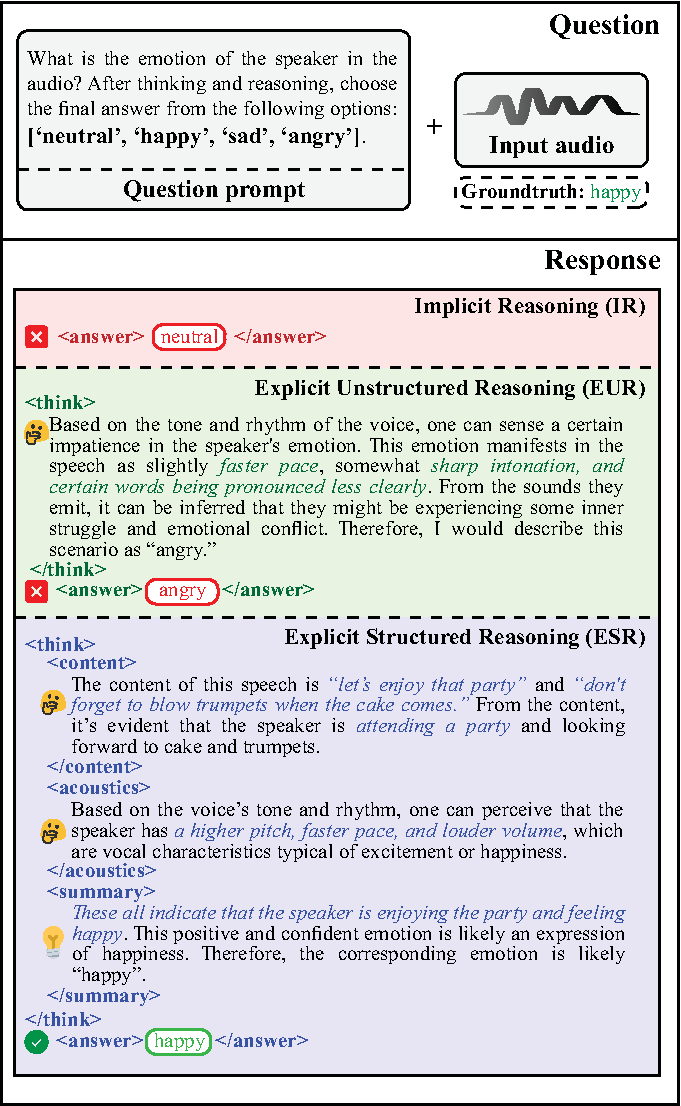
\includegraphics[width=0.49\textwidth]{img/answers.pdf}
	\caption{An example of the reasoning results of IR, EUR, and ESR}
	\label{fig:case_study}
	\vspace{-0.5cm}
\end{figure}

\subsection{Case Study}
In the Figure~\ref{fig:case_study}, we show a case study that demonstrates the response results when testing the same speech sample after training with different methods.
Models trained with IR seem to have lost many other abilities, such as not trying to think and reasoning, even though I asked them to do so.

Models trained with EUR can generate flexible reasoning based on different speech inputs. They often analyze emotions primarily through acoustic features such as pitch, rhythm, and speed. While this approach is effective for simpler cases, it faces challenges with more complex scenarios due to the omission of critical semantic emotional details.

In contrast, models trained with ESR explicitly document the speaker's key content and acoustic features, followed by a comprehensive analysis of both semantic and auditory information. This structured approach reduces the likelihood of overlooking key details, thereby enhancing the model's emotional reasoning capabilities.

\section{Conclusion}
We present EMO-RL in this paper, a novel Reinforcement Learning framework designed to enhance the emotion reasoning capabilities of Large Audio-Language Models (LALMs) in speech emotion recognition scenarios.
By incorporating emotion similarity-weighted reward, which integrates psychological prior knowledge into RL, and Explicit Structured Reasoning into our framework, EMO-RL effectively overcomes the challenges of convergence instability and limited reasoning ability in speech emotion recognition tasks.
Comprehensive experiments demonstrate that EMO-RL not only improves the emotional reasoning capabilities of LALMs on the MELD and IEMOCAP datasets (compared with SOTA, achieving an UA improvement of 25.1\% and 18.9\%, respectively), but also shows excellent generalization across different datasets.
This work signifies a step forward in applying reinforcement learning and large audio-language models to speech emotion recognition, paving the way for future speech affective computing research. Moreover, EMO-RL shows potential for enhancing multi-modal LLMs' emotion perception, bringing us closer to building truly emotional LLMs.
% Meanwhile, we explored three reasoning strategies in EMO-RL training: implicit reasoning(IR), explicit unstructured reasoning (EUR), and explicit structured reasoning (ESR).
% Experiments demonstrated that EMO-RL and ESR training strategies can significantly enhance the emotional reasoning capabilities of LALMs, achieving state-of-the-art performance on the MELD dataset with an accuracy rate of 64.5\%. Moreover, they demonstrate strong superiority in terms of generalization. EMO-RL is the first reinforcement learning framework specifically proposed for speech emotion recognition, advancing the development of speech emotion reasoning.

\section{Limitation}
% In the method, our emotion similarity matrix is designed manually based on existing prior knowledge, such as psychological principles. Therefore, in practical experiments, more optimal emotion similarity matrices may exist.  In the future, a better approach might be to dynamically adjust and optimize the emotion similarity matrix through continuous learning from experiments.
% There are some limitations of our method.
% Firstly, our EMO-RL framework is versatile enough to be applied across various multi-modal scenarios, including video, audio, and text. However, our current experiments have focused solely on speech modality without incorporating visual elements like images or videos.
% Secondly, although applying reinforcement learning to LALMs for SER tasks has achieved promising results, the computational complexity during training is relatively high, and the inference efficiency is also lower compared to previous methods. In the future, we will try to solve the above limitations.
Our proposed method has certain limitations that warrant attention.
Firstly, while our EMO-RL framework is designed to be versatile and applicable across a variety of multi-modal scenarios, including video, audio, and text, our current experimental scope has been limited to the speech modality alone. We have not yet incorporated visual elements such as images or videos into our experimental design. This restriction means that the full potential of our framework in multi-modal contexts remains unexplored.
% Future research could extend the application of EMO-RL to these additional modalities, potentially enhancing its performance and robustness in real-world scenarios where multiple modes of communication are present.
Secondly, although exploiting the LALMs for SER tasks has delivered promising results, it has also introduced challenges related to computational complexity and inference efficiency.
% The training process demands substantial computational resources, which could pose a barrier to widespread adoption, especially in contexts with limited access to high-performance computing infrastructure. 
The inference efficiency of our approach is comparatively lower than that of previous methods, which might affect its practicality for real-time applications.
In the future, we will try to solve the above limitations.

% Please add the following required packages to your document preamble:
% \usepackage{multirow}
% Please add the following required packages to your document preamble:
% \usepackage{multirow}
% \usepackage{graphicx}
% \begin{table}[]
% \resizebox{\textwidth}{!}{%
% \begin{tabular}{|c|l|l|lll|}
% \hline
% \multirow{2}{*}{Model\_Type}   & \multicolumn{1}{c|}{\multirow{2}{*}{Model}} & \multicolumn{1}{c|}{\multirow{2}{*}{Method}} & \multicolumn{3}{c|}{MELD}                                       \\ \cline{4-6} 
%                                & \multicolumn{1}{c|}{}                       & \multicolumn{1}{c|}{}                        & \multicolumn{1}{l|}{UA}    & \multicolumn{1}{l|}{WA}    & F1    \\ \hline
% \multirow{4}{*}{W/o-LALM}      & HuBERT large                                & train classification head                    & \multicolumn{1}{l|}{24.13} & \multicolumn{1}{l|}{46.37} & 24.99 \\ \cline{2-6} 
%                                & WavLM large                                 & train classification head                    & \multicolumn{1}{l|}{28.18} & \multicolumn{1}{l|}{49.31} & 29.11 \\ \cline{2-6} 
%                                & data2vec 2.0 large                          & train classification head                    & \multicolumn{1}{l|}{26.33} & \multicolumn{1}{l|}{47.72} & 27.35 \\ \cline{2-6} 
%                                & Whisper large v3                            & train classification head                    & \multicolumn{1}{l|}{31.54} & \multicolumn{1}{l|}{51.89} & 32.95 \\ \hline
% \multirow{2}{*}{LALM} & Qwen2-Audio-7B                              & Direct Inference                             & \multicolumn{1}{l|}{20.96} & \multicolumn{1}{l|}{50.69} & 20.84 \\ \cline{2-6} 
%                                & Qwen2-Audio-7B                              & Zero-Shot-COT                                & \multicolumn{1}{l|}{0}     & \multicolumn{1}{l|}{0}     & 0     \\ \hline
% \multirow{5}{*}{LALM-FT}       & Qwen2-Audio-7B                              & SFT + Prompt\textless{}1\textgreater{}       & \multicolumn{1}{l|}{0}     & \multicolumn{1}{l|}{55}    & 0     \\ \cline{2-6} 
%                                & Qwen2-Audio-7B                              & GRPO + Prompt\textless{}1\textgreater{}      & \multicolumn{1}{l|}{0}     & \multicolumn{1}{l|}{54}    & 0     \\ \cline{2-6} 
%                                & Qwen2-Audio-7B                              & EMO-RL + Prompt\textless{}1\textgreater{}    & \multicolumn{1}{l|}{0}     & \multicolumn{1}{l|}{60}    & 0     \\ \cline{2-6} 
%                                & Qwen2-Audio-7B                              & EMO-RL + Prompt\textless{}2\textgreater{}    & \multicolumn{1}{l|}{0}     & \multicolumn{1}{l|}{63}    & 0     \\ \cline{2-6} 
%                                & Qwen2-Audio-7B                              & EMO-RL + Prompt\textless{}3\textgreater{}    & \multicolumn{1}{l|}{0}     & \multicolumn{1}{l|}{69}    & 0     \\ \hline
% \end{tabular}%
% }
% \caption{}
% \label{tab:my-table}
% \end{table}

% Please add the following required packages to your document preamble:
% \usepackage{graphicx}
% \begin{table}[]
% \resizebox{\textwidth}{!}{%
% \begin{tabular}{|l|l|l|l|l|}
% \hline
% Model              & Method                                      & \multicolumn{1}{c|}{IEMOCAP} & \multicolumn{1}{c|}{RAVDESS} & SAVEE \\ \hline
% HuBERT large       & train classification head                   & 44.6                         & 25.02                        & 31.54 \\ \hline
% WavLM large        & train classification head                   & 48.59                        & 33.9                         & 34.1  \\ \hline
% data2vec 2.0 large & train classification head                   & 47.43                        & 34.21                        & 37.79 \\ \hline
% Whisper large v3   & train classification head                   & 46.14                        & 40.68                        & 42.18 \\ \hline
% Qwen2-Audio-7B     & Lora SFT + Prompt\textless{}1\textgreater{} &                              &                              &       \\ \hline
% Qwen2-Audio-7B     & GRPO + Prompt\textless{}1\textgreater{}     &                              &                              &       \\ \hline
% Qwen2-Audio-7B     & EMO-RL + Prompt\textless{}1\textgreater{}   &                              &                              &       \\ \hline
% Qwen2-Audio-7B     & EMO-RL + Prompt\textless{}2\textgreater{}   &                              &                              &       \\ \hline
% Qwen2-Audio-7B     & EMO-RL + Prompt\textless{}3\textgreater{}   &                              &                              &       \\ \hline
% \end{tabular}%
% }
% \caption{dwdwd}
% \label{tab:my-table}
% \end{table}

% \section{Preamble}
% To produce a PDF file, pdf\LaTeX{} is strongly recommended (over original \LaTeX{} plus dvips+ps2pdf or dvipdf).
% The style file \texttt{acl.sty} can also be used with
% lua\LaTeX{} and
% Xe\LaTeX{}, which are especially suitable for text in non-Latin scripts.
% The file \texttt{acl\_lualatex.tex} in this repository provides
% an example of how to use \texttt{acl.sty} with either
% lua\LaTeX{} or
% Xe\LaTeX{}.
% The first line of the file must be
% \begin{quote}
% \begin{verbatim}
% \documentclass[11pt]{article}
% \end{verbatim}
% \end{quote}

% To load the style file in the review version:
% \begin{quote}
% \begin{verbatim}
% \usepackage[review]{acl}
% \end{verbatim}
% \end{quote}
% For the final version, omit the \verb|review| option:
% \begin{quote}
% \begin{verbatim}
% \usepackage{acl}
% \end{verbatim}
% \end{quote}

% To use Times Roman, put the following in the preamble:
% \begin{quote}
% \begin{verbatim}
% \usepackage{times}
% \end{verbatim}
% \end{quote}
% (Alternatives like txfonts or newtx are also acceptable.)

% Please see the \LaTeX{} source of this document for comments on other packages that may be useful.

% Set the title and author using \verb|\title| and \verb|\author|. Within the author list, format multiple authors using \verb|\and| and \verb|\And| and \verb|\AND|; please see the \LaTeX{} source for examples.

% By default, the box containing the title and author names is set to the minimum of 5 cm. If you need more space, include the following in the preamble:
% \begin{quote}
% \begin{verbatim}
% \setlength\titlebox{<dim>}
% \end{verbatim}
% \end{quote}
% where \verb|<dim>| is replaced with a length. Do not set this length smaller than 5 cm.

% \section{Document Body}

% \subsection{Footnotes}

% Footnotes are inserted with the \verb|\footnote| command.\footnote{This is a footnote.}

% \subsection{Tables and figures}

% See Table~\ref{tab:accents} for an example of a table and its caption.
% \textbf{Do not override the default caption sizes.}

% \begin{table}
%   \centering
%   \begin{tabular}{lc}
%     \hline
%     \textbf{Command} & \textbf{Output} \\
%     \hline
%     \verb|{\"a}|     & {\"a}           \\
%     \verb|{\^e}|     & {\^e}           \\
%     \verb|{\`i}|     & {\`i}           \\
%     \verb|{\.I}|     & {\.I}           \\
%     \verb|{\o}|      & {\o}            \\
%     \verb|{\'u}|     & {\'u}           \\
%     \verb|{\aa}|     & {\aa}           \\\hline
%   \end{tabular}
%   \begin{tabular}{lc}
%     \hline
%     \textbf{Command} & \textbf{Output} \\
%     \hline
%     \verb|{\c c}|    & {\c c}          \\
%     \verb|{\u g}|    & {\u g}          \\
%     \verb|{\l}|      & {\l}            \\
%     \verb|{\~n}|     & {\~n}           \\
%     \verb|{\H o}|    & {\H o}          \\
%     \verb|{\v r}|    & {\v r}          \\
%     \verb|{\ss}|     & {\ss}           \\
%     \hline
%   \end{tabular}
%   \caption{Example commands for accented characters, to be used in, \emph{e.g.}, Bib\TeX{} entries.}
%   \label{tab:accents}
% \end{table}

% As much as possible, fonts in figures should conform
% to the document fonts. See Figure~\ref{fig:experiments} for an example of a figure and its caption.

% Using the \verb|graphicx| package graphics files can be included within figure
% environment at an appropriate point within the text.
% The \verb|graphicx| package supports various optional arguments to control the
% appearance of the figure.
% You must include it explicitly in the \LaTeX{} preamble (after the
% \verb|\documentclass| declaration and before \verb|\begin{document}|) using
% \verb|\usepackage{graphicx}|.

% \begin{figure}[t]
%   \includegraphics[width=\columnwidth]{example-image-golden}
%   \caption{A figure with a caption that runs for more than one line.
%     Example image is usually available through the \texttt{mwe} package
%     without even mentioning it in the preamble.}
%   \label{fig:experiments}
% \end{figure}

% \begin{figure*}[t]
%   \includegraphics[width=0.48\linewidth]{example-image-a} \hfill
%   \includegraphics[width=0.48\linewidth]{example-image-b}
%   \caption {A minimal working example to demonstrate how to place
%     two images side-by-side.}
% \end{figure*}

% \subsection{Hyperlinks}

% Users of older versions of \LaTeX{} may encounter the following error during compilation:
% \begin{quote}
% \verb|\pdfendlink| ended up in different nesting level than \verb|\pdfstartlink|.
% \end{quote}
% This happens when pdf\LaTeX{} is used and a citation splits across a page boundary. The best way to fix this is to upgrade \LaTeX{} to 2018-12-01 or later.

% \subsection{Citations}

% \begin{table*}
%   \centering
%   \begin{tabular}{lll}
%     \hline
%     \textbf{Output}           & \textbf{natbib command} & \textbf{ACL only command} \\
%     \hline
%     ~\citep{Gusfield:97}       & \verb|~\citep|           &                           \\
%     \citealp{Gusfield:97}     & \verb|\citealp|         &                           \\
%     \citet{Gusfield:97}       & \verb|\citet|           &                           \\
%     \citeyearpar{Gusfield:97} & \verb|\citeyearpar|     &                           \\
%     ~\citeposs{Gusfield:97}    &                         & \verb|~\citeposs|          \\
%     \hline
%   \end{tabular}
%   \caption{\label{citation-guide}
%     Citation commands supported by the style file.
%     The style is based on the natbib package and supports all natbib citation commands.
%     It also supports commands defined in previous ACL style files for compatibility.
%   }
% \end{table*}

% Table~\ref{citation-guide} shows the syntax supported by the style files.
% We encourage you to use the natbib styles.
% You can use the command \verb|\citet| (cite in text) to get ``author (year)'' citations, like this citation to a paper by \citet{Gusfield:97}.
% You can use the command \verb|~\citep| (cite in parentheses) to get ``(author, year)'' citations ~\citep{Gusfield:97}.
% You can use the command \verb|\citealp| (alternative cite without parentheses) to get ``author, year'' citations, which is useful for using citations within parentheses (e.g. \citealp{Gusfield:97}).

% A possessive citation can be made with the command \verb|~\citeposs|.
% This is not a standard natbib command, so it is generally not compatible
% with other style files.

% \subsection{References}

% \nocite{Ando2005,andrew2007scalable,rasooli-tetrault-2015}

% The \LaTeX{} and Bib\TeX{} style files provided roughly follow the American Psychological Association format.
% If your own bib file is named \texttt{custom.bib}, then placing the following before any appendices in your \LaTeX{} file will generate the references section for you:
% \begin{quote}
% \begin{verbatim}
% \bibliography{custom}
% \end{verbatim}
% \end{quote}

% You can obtain the complete ACL Anthology as a Bib\TeX{} file from \url{https://aclweb.org/anthology/anthology.bib.gz}.
% To include both the Anthology and your own .bib file, use the following instead of the above.
% \begin{quote}
% \begin{verbatim}
% \bibliography{anthology,custom}
% \end{verbatim}
% \end{quote}

% Please see Section~\ref{sec:bibtex} for information on preparing Bib\TeX{} files.

% \subsection{Equations}

% An example equation is shown below:
% \begin{equation}
%   \label{eq:example}
%   A = \pi r^2
% \end{equation}

% Labels for equation numbers, sections, subsections, figures and tables
% are all defined with the \verb|\label{label}| command and cross references
% to them are made with the \verb|\ref{label}| command.

% This an example cross-reference to Equation~\ref{eq:example}.

% \subsection{Appendices}

% Use \verb|\appendix| before any appendix section to switch the section numbering over to letters. See Appendix~\ref{sec:appendix} for an example.

% \section{Bib\TeX{} Files}
% \label{sec:bibtex}

% Unicode cannot be used in Bib\TeX{} entries, and some ways of typing special characters can disrupt Bib\TeX's alphabetization. The recommended way of typing special characters is shown in Table~\ref{tab:accents}.

% Please ensure that Bib\TeX{} records contain DOIs or URLs when possible, and for all the ACL materials that you reference.
% Use the \verb|doi| field for DOIs and the \verb|url| field for URLs.
% If a Bib\TeX{} entry has a URL or DOI field, the paper title in the references section will appear as a hyperlink to the paper, using the hyperref \LaTeX{} package.

% \section*{Limitations}

% Since December 2023, a "Limitations" section has been required for all papers submitted to ACL Rolling Review (ARR). This section should be placed at the end of the paper, before the references. The "Limitations" section (along with, optionally, a section for ethical considerations) may be up to one page and will not count toward the final page limit. Note that these files may be used by venues that do not rely on ARR so it is recommended to verify the requirement of a "Limitations" section and other criteria with the venue in question.

% \section*{Acknowledgments}

% This document has been adapted
% by Steven Bethard, Ryan Cotterell and Rui Yan
% from the instructions for earlier ACL and NAACL proceedings, including those for
% ACL 2019 by Douwe Kiela and Ivan Vuli\'{c},
% NAACL 2019 by Stephanie Lukin and Alla Roskovskaya,
% ACL 2018 by Shay Cohen, Kevin Gimpel, and Wei Lu,
% NAACL 2018 by Margaret Mitchell and Stephanie Lukin,
% Bib\TeX{} suggestions for (NA)ACL 2017/2018 from Jason Eisner,
% ACL 2017 by Dan Gildea and Min-Yen Kan,
% NAACL 2017 by Margaret Mitchell,
% ACL 2012 by Maggie Li and Michael White,
% ACL 2010 by Jing-Shin Chang and Philipp Koehn,
% ACL 2008 by Johanna D. Moore, Simone Teufel, James Allan, and Sadaoki Furui,
% ACL 2005 by Hwee Tou Ng and Kemal Oflazer,
% ACL 2002 by Eugene Charniak and Dekang Lin,
% and earlier ACL and EACL formats written by several people, including
% John Chen, Henry S. Thompson and Donald Walker.
% Additional elements were taken from the formatting instructions of the \emph{International Joint Conference on Artificial Intelligence} and the \emph{Conference on Computer Vision and Pattern Recognition}.

% % Bibliography entries for the entire Anthology, followed by custom entries
% %\bibliography{anthology,custom}
% % Custom bibliography entries only
% \bibliography{custom}

% \appendix

% \section{Example Appendix}
% \label{sec:appendix}

% This is an appendix.
\bibliography{custom}
\end{document}
